% WACV 2027 draft — condensed from the MEng final report.
% TODO: port into the official WACV 2027 author kit and anonymise.
% Build:  lualatex -> biber -> lualatex  (from this directory)

\documentclass[10pt,twocolumn,letterpaper]{article}

\usepackage[top=1in,bottom=1in,left=0.8in,right=0.8in,columnsep=0.3125in]{geometry}
\usepackage{newtxtext,newtxmath} % Times-like, as WACV
\usepackage{graphicx}
\usepackage{booktabs}
\usepackage{amsmath}
\usepackage{multirow}
\usepackage{xcolor}
\usepackage[style=ieee,backend=biber,maxnames=6]{biblatex}
\addbibresource{../report/references.bib}
\usepackage[colorlinks=true,linkcolor=blue,citecolor=blue,urlcolor=blue]{hyperref}

\graphicspath{{../report/imgs/}{../report/imgs/}}

% Visible work-remaining markers
\newcommand{\TODO}[1]{\textcolor{red}{\textbf{[TODO: #1]}}}

\pagestyle{plain}

\title{\Large\bf Edge-Deployable NIR-to-RGB Translation as a Pre-Processor\\ for Frozen RGB Vision Models}
\author{\TODO{authors}}
\date{}

\begin{document}
\maketitle

%-------------------------------------------------------------------------
\begin{abstract}
Modern vision models are trained almost entirely on visible-band RGB imagery and degrade badly on near-infrared (NIR) input. Retraining every downstream model on NIR data is rarely practical. We develop an NIR$\rightarrow$RGB translator that sits between an NIR sensor and an unmodified, frozen RGB model, and judge it by a stricter criterion than image quality: how much of each frozen model's native-RGB behaviour the translation recovers. To obtain supervision, a shared-aperture beam-splitter rig captured 12{,}536 simultaneous, homography-aligned NIR/RGB pairs. On this data a 116M-parameter NAFNet teacher is trained with feature-matching losses against frozen foundation models (DINOv2, CLIP, ResNet-50) in place of the conventional single perceptual term, then distilled into a 1.7M-parameter student ($67.3\times$ reduction) and exported as a deterministic 2.3MB mixed-INT8 artefact. Both the student and its quantised export achieve positive gap closure on all five downstream tasks spanning detection, segmentation and depth, and the deployed student runs at 5\,FPS on a Raspberry~Pi~5 CPU and 27\,FPS on its Hailo-8L accelerator. A Pix2Pix baseline that matches the student on PSNR and SSIM recovers almost none of this downstream behaviour, showing that feature-space supervision and behaviour-centred evaluation, not pixel fidelity, are what make a translation pre-processor useful. The dataset will be released publicly.
\end{abstract}

%-------------------------------------------------------------------------
\section{Introduction}
\label{sec:intro}

Near-infrared (NIR) imaging is standard in biometrics, agriculture, surveillance and night operation, but the dominant vision toolchain of detectors, segmenters and depth estimators is trained almost entirely on visible-band RGB. On NIR input these models degrade badly: colour is absent, material appearance changes (foliage is bright, water dark, skin smooth), and features tuned to RGB statistics stop firing. Retraining every downstream model on labelled NIR data is rarely practical.

A practical remedy is a learned NIR$\rightarrow$RGB translator placed between the sensor and the frozen RGB model. Most prior translation work, however, is optimised and evaluated for image fidelity (PSNR, SSIM, LPIPS) or human-judged realism. Our central finding is that these criteria do not predict usefulness as a pre-processor: a conventional Pix2Pix baseline~\cite{isola2017image} that \emph{ties our compact student on PSNR and SSIM} leaves downstream behaviour at --- and on detection, below --- the level of feeding the frozen models raw NIR.

We therefore make downstream behaviour the training signal and the success criterion. A NAFNet~\cite{chen2022nafnet} teacher is supervised by feature matching against an ensemble of frozen foundation models (DINOv2~\cite{oquab2024dinov2}, CLIP~\cite{radford2021clip}, ResNet-50~\cite{he2016resnet}) in place of the single VGG perceptual term, and evaluated with a \emph{gap-closure} harness that measures, for each frozen downstream model, how far translation moves its outputs from raw-NIR behaviour toward native-RGB behaviour. Because paired NIR/RGB supervision at scale does not exist publicly with true simultaneity, we built a shared-aperture beam-splitter rig around a Raspberry~Pi that captures both bands through a common optical centre, yielding 12{,}536 homography-aligned pairs.

Our contributions are:
\begin{enumerate}
  \item \textbf{Dataset and rig.} A low-cost shared-aperture capture rig producing simultaneous NIR/RGB pairs related by a single depth-independent homography, and a 12{,}536-pair aligned urban dataset, which will be released publicly (Sec.~\ref{sec:dataset}). \TODO{add dataset link}
  \item \textbf{Foundation-ensemble supervision.} Replacing the VGG perceptual loss with simultaneous feature matching against DINOv2, CLIP and ResNet-50, with checkpoint selection by validation CLIP cosine rather than PSNR (Sec.~\ref{sec:method}). An ablation shows this term drives the downstream gains.
  \item \textbf{Behaviour-centred evaluation.} An annotation-free gap-closure harness across two detectors, two segmentation distributions, depth and embedding probes, with independent probes (DINOv2-L, SigLIP2) held out of every training objective (Sec.~\ref{sec:eval}).
  \item \textbf{Edge deployment.} A distillation and mixed-INT8 export path producing a 1.7M-parameter, 2.3MB deterministic artefact at 5\,FPS on the Raspberry~Pi~5 CPU and 27\,FPS on the Hailo-8L NPU (Sec.~\ref{sec:edge}).
\end{enumerate}

%-------------------------------------------------------------------------
\section{Related work}
\label{sec:related}

\paragraph{Paired image translation.} Pix2Pix~\cite{isola2017image} established the conditional-GAN formulation for paired translation; Pix2PixHD~\cite{wang2018pix2pixhd} added coarse-to-fine generation and discriminator feature matching, and SPADE~\cite{park2019spade} semantic conditioning. Perceptual losses on frozen network features~\cite{johnson2016perceptual} are the standard remedy for L1 blur. Diffusion models~\cite{ho2020denoising,saharia2022image} capture the one-to-many ambiguity of colourisation but their iterative, stochastic sampling conflicts with a deterministic real-time pre-processor.

\paragraph{Cross-spectral translation.} The closest prior work, Pix2Next~\cite{pix2next2024}, injects features of a single frozen foundation model into a Pix2PixHD-style generator for RGB$\rightarrow$NIR and evaluates on one downstream detector. We reverse the direction, use a foundation \emph{ensemble} purely as a training loss on an unmodified restoration backbone, and generalise downstream evaluation to a task-spanning panel. Image-translation-based domain adaptation (e.g.\ CyCADA~\cite{hoffman2018cycada}) shares our framing of translation as input-distribution alignment. \TODO{cite recent NIR colourisation work and compare against one}

\paragraph{Restoration backbones and edge deployment.} NAFNet~\cite{chen2022nafnet} reaches state-of-the-art restoration with an activation-free block whose small operator set suits INT8 export~\cite{jacob2018quantization,gholami2021survey}. To our knowledge it has not previously been used for NIR$\rightarrow$RGB synthesis; prior work in this direction relies on conditional GANs or diffusion. Knowledge distillation~\cite{hinton2015distilling,romero2015fitnets} closes the gap between training-time capacity and deployment budget.

\paragraph{Paired NIR/RGB data.} Public paired sets such as the EPFL RGB--NIR scene dataset~\cite{brown2011multispectral,epfl_rgbnir_dataset} use sequential exposures, so moving content (pedestrians, vehicles, foliage) mismatches between bands, corrupting supervised pairs. Our rig removes this by capturing both bands simultaneously through one aperture.

%-------------------------------------------------------------------------
\section{A simultaneous, homography-aligned NIR/RGB dataset}
\label{sec:dataset}

\begin{figure}[t]
\centering
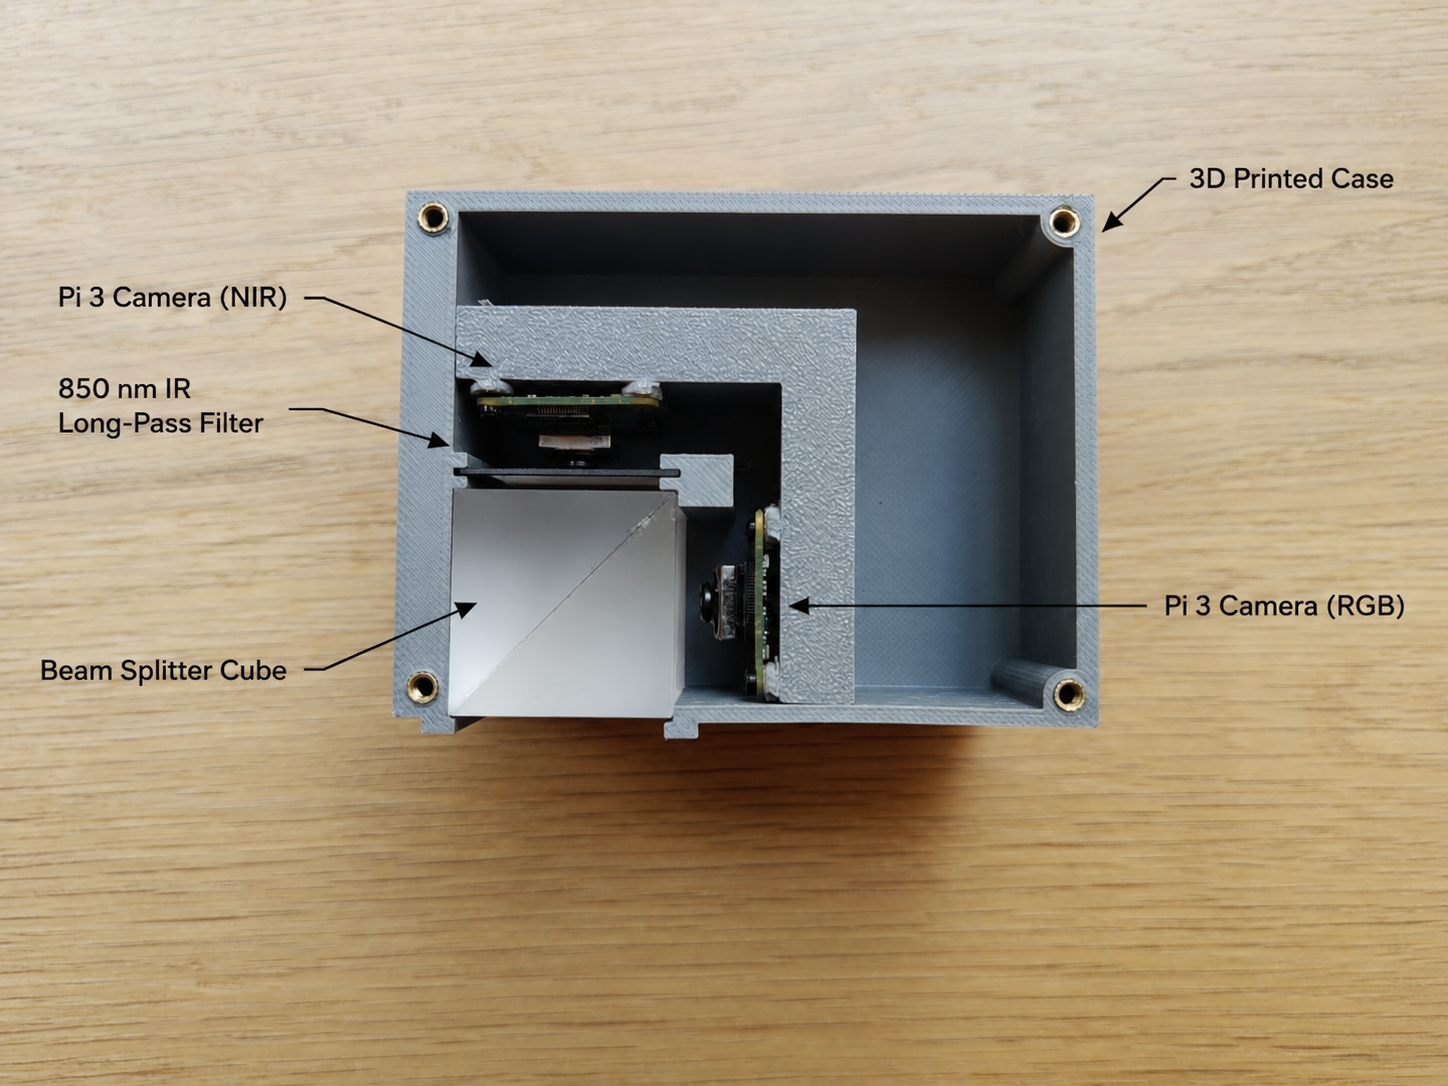
\includegraphics[width=0.99\linewidth]{device-labeled.png}
\caption{The capture rig. A beam-splitter cube feeds one shared aperture to an RGB camera and an NIR camera behind an 850\,nm long-pass filter, giving both sensors a common optical centre; residual differences are absorbed by a per-pair homography.}
\label{fig:rig}
\end{figure}

Two cameras separated by a baseline cannot share an optical centre, so parallax rules out any single 2D warp aligning all depths. We solve this optically: a beam-splitter cube divides incoming light between two Raspberry~Pi Camera Module~3 sensors, one behind an 850\,nm long-pass filter (Fig.~\ref{fig:rig}). Both bands are captured at the same instant through a shared aperture, so every pair is free of temporal content mismatch and related by a single depth-independent homography.

Data was collected over 20+ hours of cycling through London with the rig backpack-mounted, one pair every 5\,s. Pairs are filtered for sharpness (variance of Laplacian $>100$), centre-cropped, aligned by SIFT matches with Lowe's ratio test and a RANSAC homography, cropped to the valid overlap, and resized to $256\times256$. This yields \textbf{12{,}536} aligned pairs, split 80/10/10 at image level (10{,}028/1{,}253/1{,}255) with a fixed seed. The rig was tilted upward and the output resolution chosen so pedestrians are not identifiable; capture and processing excluded personally identifiable information. The dataset will be released publicly.

%-------------------------------------------------------------------------
\section{Method}
\label{sec:method}

\subsection{Teacher: NAFNet with foundation-ensemble supervision}

The translator is a width-64 NAFNet (116M parameters): a U-shaped encoder--bottleneck--decoder of activation-free NAFBlocks with $[2,2,4,8]$ encoder blocks, a 12-block bottleneck and additive skips, ending in $\tanh$. The global input$\rightarrow$output residual is disabled because input and output are different modalities. The backbone was chosen for deployment reasons: its operator set (convolution, LayerNorm, elementwise multiply, PixelShuffle) exports cleanly and its lack of saturating nonlinearities behaves predictably under INT8 quantisation.

The training objective keeps a strong L1 colour anchor (weight 20), an MS-SSIM term~\cite{wang2003msssim} (3) and a lightly weighted LSGAN PatchGAN term (0.3), and replaces the conventional VGG perceptual term with a \emph{foundation-model feature-matching ensemble}: for frozen extractors $F$ (DINOv2 ViT-S/14, weight 40; CLIP ViT-B/32, weight 20; ResNet-50, weight 5), training pushes $F(T(x_{\text{NIR}}))\approx F(x_{\text{RGB}})$ at $224\times224$. The intuition is direct: a downstream model whose predictions depend on features like $F(\cdot)$ behaves on $T(x_{\text{NIR}})$ more like it does on $x_{\text{RGB}}$. Adversarial and ensemble weights warm up over 30 epochs; training runs 200 epochs from scratch (Adam, lr $2\times10^{-5}$, batch 1, FP32) and the checkpoint is selected by validation CLIP cosine similarity, not PSNR.

\subsection{Student: feature-distilled edge model}
\label{sec:student}

A width-16 NAFNet student (1.7M parameters, $67.3\times$ smaller; encoder $[1,1,1,2]$, 2 middle blocks) is distilled from the teacher. The dominant term is an L1 loss to the teacher's output (weight 50) with a light ground-truth L1 anchor (5), so colour stays tied to measured RGB while teacher artefacts are not amplified. Auxiliary feature-matching terms to the ground truth cover generic and task-facing representations --- DINOv2 (40), CLIP (20), ResNet-50 (5), SegFormer-B0 (15) and DepthAnything-Small (10) --- plus a feature-level KD term between student and teacher outputs (0.5). The checkpoint is selected by validation CLIP cosine similarity (0.8585 at epoch 99).

\subsection{Edge export}
\label{sec:export}

The FP32 student exports to LiteRT via litert-torch (direct PyTorch lowering; an onnx2tf path mis-shaped LayerNorm reductions) and is post-training quantised to mixed INT8: per-channel weights, MinMax activations from 100 training-split calibration frames, with PixelShuffle/LayerNorm-adjacent ops left in FP32. A second path recompiles the ONNX graph to a Hailo-8L HEF, requiring three numerically exact operator rewrites (explicit kernel shapes; SimpleGate as identity-selector convolutions; two-stage global pooling).

%-------------------------------------------------------------------------
\section{Evaluation protocol}
\label{sec:eval}

Image-quality metrics are reported as sanity checks, but the primary criterion is behavioural. A panel of frozen RGB-pretrained models is run on raw NIR, translated RGB and native RGB, and each task reports
\[
\text{gap closure} = \frac{m(\text{translated}) - m(\text{nir})}{m(\text{rgb}) - m(\text{nir})},
\]
where $m$ is the task's agreement metric with the native-RGB prediction (sign-adjusted for lower-is-better metrics): 0 means no better than raw NIR, 1 means native-RGB behaviour fully recovered, negative values mean translation harms the task. The five primary tasks are YOLOv8m~\cite{jocher2023yolov8} and RT-DETR-L~\cite{zhao2024rtdetr} detection (mAP@0.5 against native-RGB pseudo-labels), SegFormer-B0~\cite{xie2021segformer} segmentation on ADE20K~\cite{zhou2017ade20k} and Cityscapes~\cite{cordts2016cityscapes} distributions (class-mean Dice), and DepthAnything-Small~\cite{yang2024depthanything} (per-image min--max-normalised L1). DINOv2-L and SigLIP2~\cite{tschannen2025siglip2} cosine agreement are supporting embedding probes that appear in no training objective; DINOv2-S and CLIP-family scores are treated as supporting evidence only, since related backbones supplied training losses. The harness is verified by oracle fixtures (identity, negative-control, zero-denominator, ordering) and per-image results are retained for image-level bootstrap confidence intervals. These numbers measure recovery of native-RGB \emph{model behaviour}; native-RGB predictions act as the behavioural reference.

%-------------------------------------------------------------------------
\section{Results}
\label{sec:results}

All numbers are on the full 1{,}255-pair held-out test split. \TODO{rerun with more seeds}

\subsection{Image quality does not separate the methods}

\begin{table}[t]
\centering
\footnotesize
\setlength{\tabcolsep}{3.5pt}
\begin{tabular}{lcccc}
\toprule
\textbf{Model} & \textbf{PSNR}$\uparrow$ & \textbf{SSIM}$\uparrow$ & \textbf{LPIPS}$\downarrow$ & \textbf{Params} \\
\midrule
Raw NIR & 16.65 & 0.656 & 0.337 & --- \\
Pix2Pix~\cite{isola2017image} & 24.03 & 0.752 & 0.185 & 54.4M \\
Teacher (NAFNet-64) & 26.16 & 0.818 & 0.103 & 116M \\
Student FP32 (NAFNet-16) & 24.09 & 0.781 & 0.146 & 1.7M \\
Student mixed-INT8 & 23.57 & 0.770 & 0.153 & 1.7M \\
\bottomrule
\end{tabular}
\caption{Image quality on the held-out test split. The 1.7M-parameter student ties the 54.4M-parameter Pix2Pix baseline on PSNR and beats it on SSIM/LPIPS --- yet Tab.~\ref{tab:closure} shows they behave completely differently downstream.}
\label{tab:quality}
\end{table}

Table~\ref{tab:quality} shows the teacher strongest on all fidelity metrics and the width-16 student tying Pix2Pix on PSNR (24.09 vs 24.03) while beating it on SSIM (0.781 vs 0.752) and LPIPS (0.146 vs 0.185) at $1/32$ of the parameters. Quantisation costs a further 0.52\,dB PSNR for a $3.1\times$ smaller artefact. On classic metrics the student and Pix2Pix are interchangeable, which is exactly why classic metrics are insufficient.

\subsection{Downstream behaviour separates them completely}

\begin{table*}[t]
\centering
\footnotesize
\setlength{\tabcolsep}{4.5pt}
\begin{tabular}{llccccccc}
\toprule
& & & \textbf{Pix2Pix} & \textbf{Teacher} & \multicolumn{2}{c}{\textbf{Student FP32}} & \multicolumn{2}{c}{\textbf{Student INT8}} \\
\cmidrule(lr){6-7}\cmidrule(lr){8-9}
\textbf{Task} & \textbf{Metric} & \textbf{Raw NIR} & closure & closure & value & closure & value & closure \\
\midrule
Detection & YOLOv8m mAP@0.5 & 0.224 & $-0.152$ & $+0.108$ & 0.284 & $+0.077$ & 0.288 & $+0.083$ \\
Detection & RT-DETR-L mAP@0.5 & 0.243 & $-0.125$ & $+0.194$ & 0.297 & $+0.072$ & 0.283 & $+0.053$ \\
Segmentation & ADE20K class-mean Dice & 0.694 & $+0.183$ & $+0.670$ & 0.874 & $+0.587$ & 0.868 & $+0.569$ \\
Segmentation & Cityscapes class-mean Dice & 0.447 & $+0.226$ & $+0.463$ & 0.642 & $+0.351$ & 0.619 & $+0.311$ \\
Depth & DepthAnything norm.\ L1 $\downarrow$ & 0.677 & $-0.001$ & $+0.461$ & 0.424 & $+0.374$ & 0.455 & $+0.328$ \\
\midrule
Embedding & DINOv2-L cosine & 0.728 & $-0.020$ & $+0.708$ & 0.882 & $+0.566$ & 0.871 & $+0.525$ \\
Embedding & SigLIP2 cosine & 0.883 & $+0.095$ & $+0.675$ & 0.946 & $+0.538$ & 0.943 & $+0.511$ \\
\bottomrule
\end{tabular}
\caption{Gap closure toward native-RGB behaviour on the held-out test split. Embedding probes (DINOv2-L, SigLIP2) appear in no training objective. Pix2Pix, which ties the student on pixel metrics, is at or below raw-NIR behaviour on detection, depth and DINOv2-L, while both student precisions stay positive on all five primary tasks.}
\label{tab:closure}
\end{table*}

Table~\ref{tab:closure} is the paper's central result. Both student precisions achieve positive closure on all five primary tasks: detection $+0.077$/$+0.072$ (FP32), segmentation $+0.587$/$+0.351$, depth $+0.374$, with independent-embedding closures of $+0.566$ (DINOv2-L) and $+0.538$ (SigLIP2); mixed-INT8 export keeps every closure positive. Pix2Pix --- the student's pixel-metric equal --- closes essentially nothing: DINOv2-L cosine 0.723 versus 0.728 for doing no translation at all, depth agreement identical to raw NIR, and detection \emph{below} the raw-NIR baseline ($-0.152$, $-0.125$). Recovery is uneven: detection closures are several times smaller than segmentation and depth, plausibly because detection depends on small objects and fine texture, which translation reproduces least faithfully.

\begin{figure}[t]
\centering
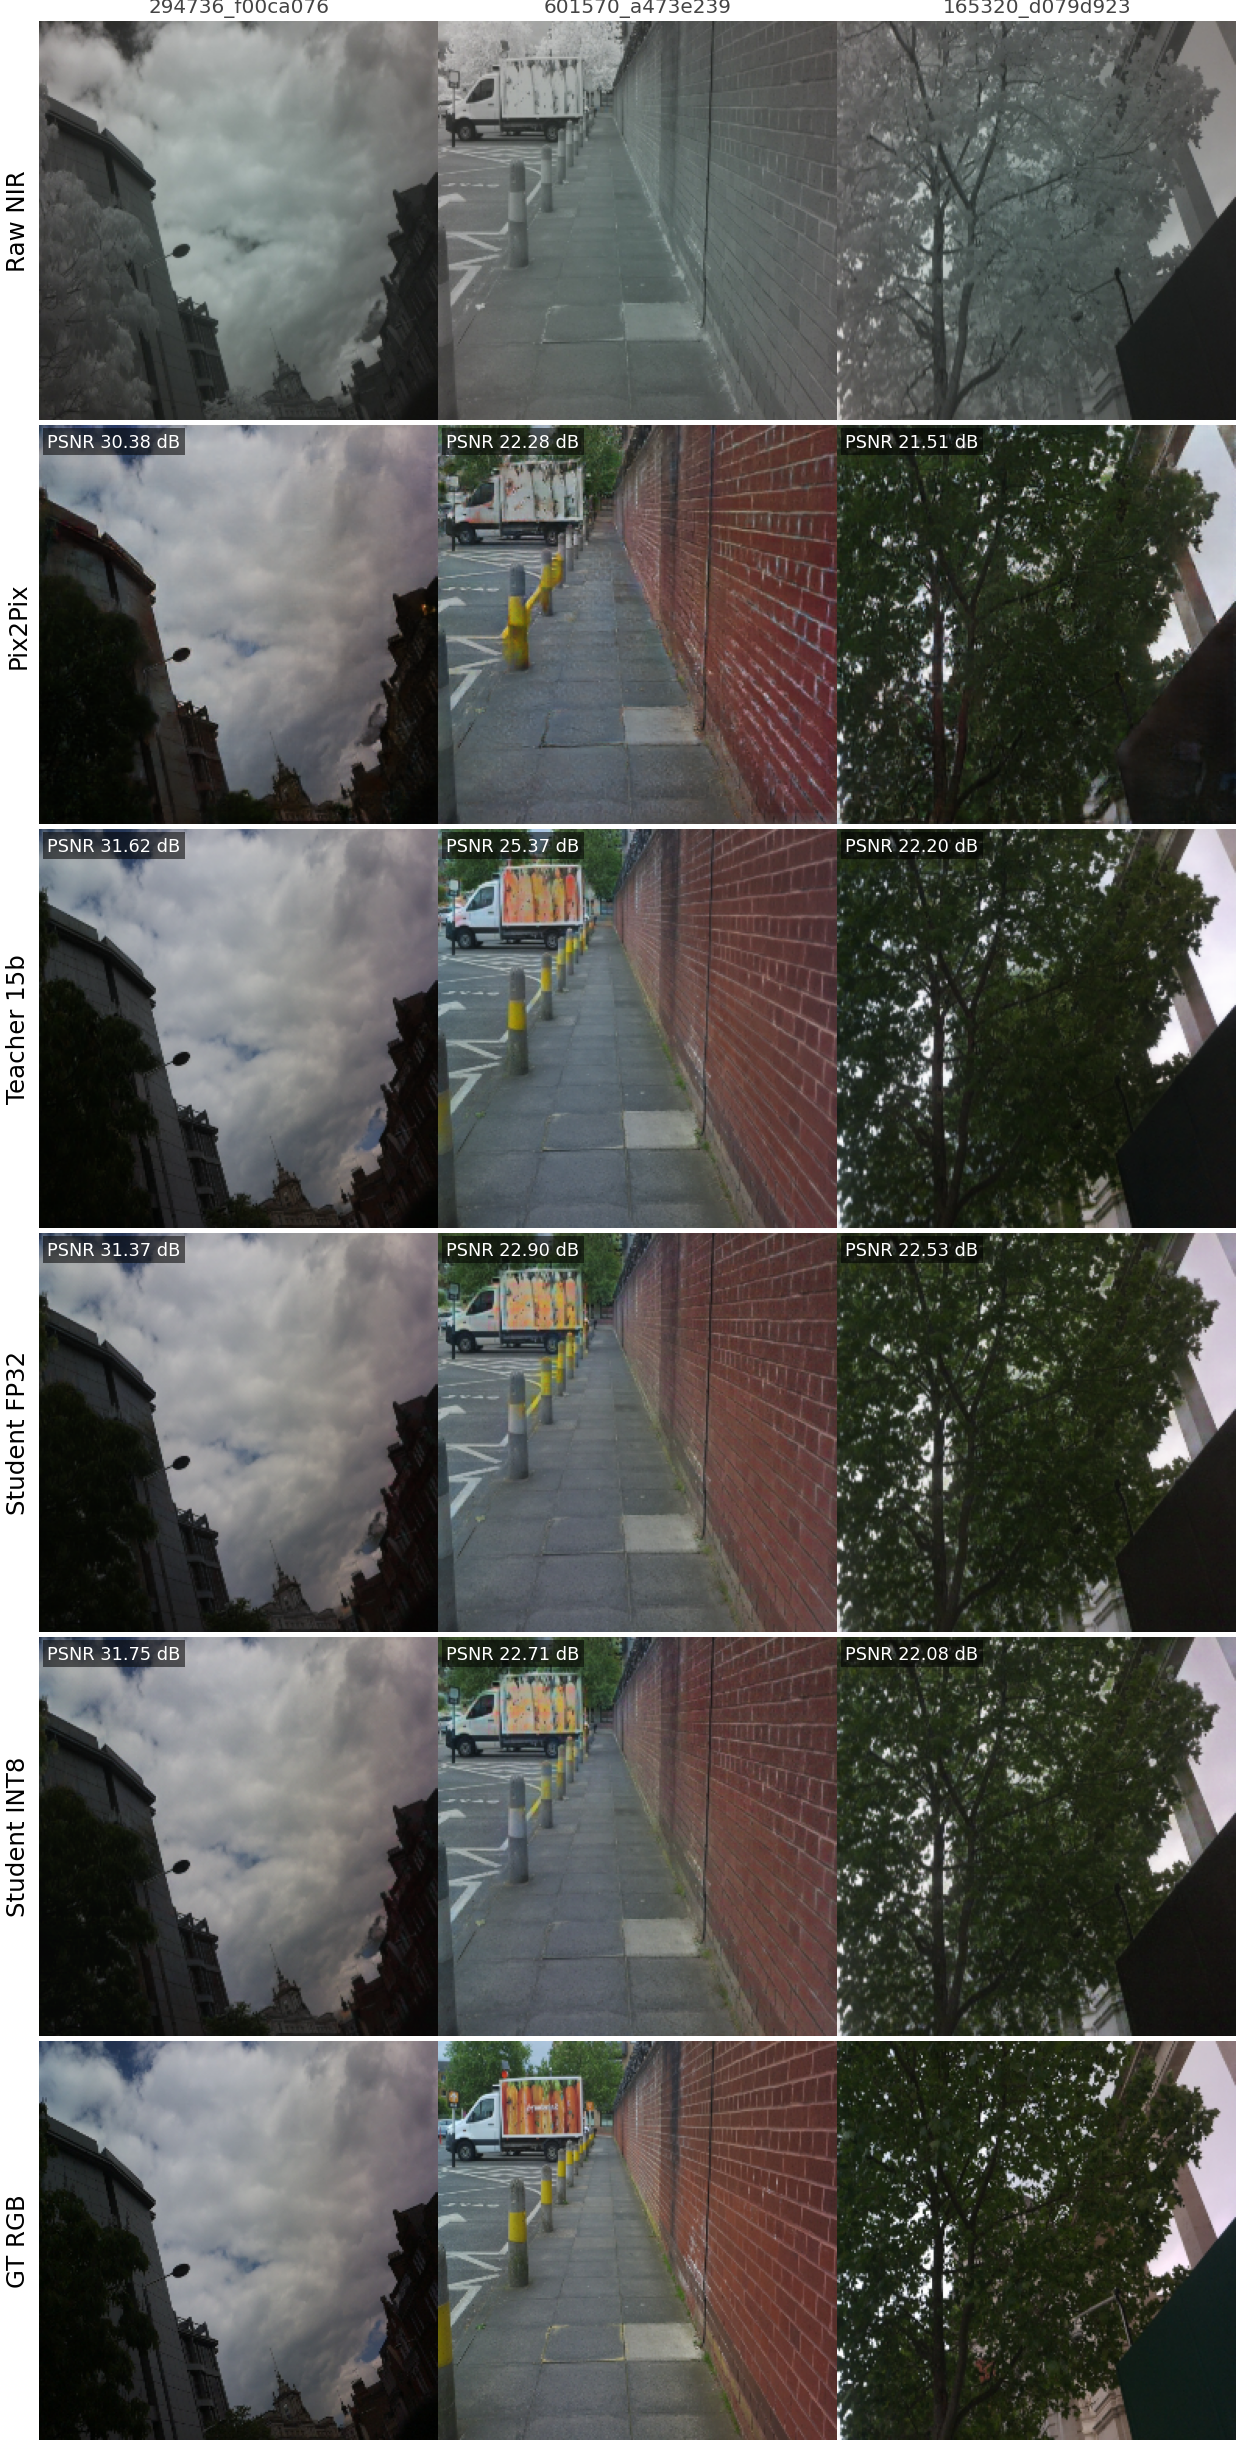
\includegraphics[width=0.99\linewidth]{random_no_people_grid.png}
\caption{Random held-out samples. Rows, top to bottom: raw NIR, Pix2Pix, teacher, student FP32, student INT8, ground-truth RGB.}
\label{fig:qual}
\end{figure}

\subsection{Ablations}

\begin{table}[t]
\centering
\footnotesize
\setlength{\tabcolsep}{2.7pt}
\begin{tabular}{lccccc}
\toprule
\textbf{Teacher config} & \textbf{PSNR} & \textbf{DINOv2-L} & \textbf{YOLO cl.} & \textbf{ADE cl.} & \textbf{Depth} \\
\midrule
No FM ensemble & \textbf{27.10} & 0.886 & $+0.011$ & $+0.619$ & 0.420 \\
No GAN & 26.33 & \textbf{0.923} & $+0.077$ & $+0.667$ & \textbf{0.347} \\
No MS-SSIM & 26.29 & 0.922 & $+0.076$ & $+0.653$ & 0.348 \\
No FM warm-up & 26.31 & 0.921 & $+0.064$ & $+0.665$ & 0.353 \\
Full objective & 26.16 & 0.921 & $+\textbf{0.108}$ & $+\textbf{0.670}$ & 0.365 \\
\bottomrule
\end{tabular}
\caption{Teacher ablations. Removing the foundation ensemble (No FM) \emph{raises} PSNR while collapsing detection closure and weakening embedding agreement: pixel fidelity and downstream utility move in opposite directions.}
\label{tab:ablation}
\end{table}

Table~\ref{tab:ablation} isolates the loss components. Removing the foundation ensemble gives the \emph{best} PSNR (27.10\,dB) and the \emph{worst} downstream behaviour (YOLO closure $+0.011$, DINOv2-L 0.886), confirming the ensemble drives the downstream gains and that optimising pixel fidelity actively competes with them. GAN, MS-SSIM and warm-up ablations sit within confidence intervals on most probes; the adversarial term earns its place on detection ($+0.077\rightarrow+0.108$). \TODO{try pix2pix with the ensemble loss}

Student-side ablations (same NAFNet-16 backbone, different auxiliary supervision) show that adding task-facing feature terms and teacher feature-KD to a DINOv2/CLIP-only recipe improves nearly every probe; the selected feature-KD variant is best on LPIPS, both embedding probes, both segmentation means and YOLO.

\subsection{Edge deployment}
\label{sec:edge}

On the Raspberry~Pi~5, the mixed-INT8 LiteRT student runs at 198\,ms (5.05\,FPS) per $256\times256$ frame on the 4-thread CPU (FP32: 4.40\,FPS; quantisation is what reaches the target) and 36.3\,ms (27.2\,FPS) on the Hailo-8L NPU; a width-32 variant reaches 10.8\,FPS on the NPU. The INT8 artefact is 2.3\,MB, peak inference memory under 50\,MB, with no swap or thermal throttling over sustained runs, and output is bit-exact deterministic across repeated runs. The CPU margin is slim (p95 221\,ms exceeds the 200\,ms budget), so the NPU is the recommended backend.

A controlled robustness sweep on the NIR input defines the operating envelope: exposure and gamma shifts of $\pm20\%$ cost at most 1.14\,dB PSNR, while Gaussian blur at $\sigma{=}2$ or noise at $\sigma{=}0.03$ degrade embedding agreement below the raw-NIR level, so deployment should monitor input sharpness and noise and reject degraded frames.

\subsection{Transfer to other modalities}

The recipe is not NIR-specific. On KAIST thermal~\cite{hwang2015multispectral} it transfers unchanged (CLIP cosine 0.924 vs 0.46 raw; static scene classes improve strongly, while the person class fails because thermal's pedestrian contrast is spent on global colour synthesis). On SAR (WHU-OPT-SAR-derived pairs~\cite{li2022whuoptsar}) it breaks down: pixel metrics collapse and downstream gains are marginal (EuroSAT~\cite{helber2019eurosat} 0.165$\rightarrow$0.425, RemoteCLIP~\cite{liu2024remoteclip} 0.759). The approach applies where the source modality shares spectral structure with RGB; it is not a universal cross-modal adapter.

%-------------------------------------------------------------------------
\section{Limitations}
\label{sec:limitations}

The downstream panel measures behavioural agreement with frozen-model native-RGB outputs, which is the deployment-relevant quantity for reusing an existing RGB stack. The dataset is outdoor urban London on one rig; indoor, rural and other-climate generalisation is not established, and privacy-preserving capture precludes person-centric evaluation (face, re-ID, pose) --- notable since person is among the weaker classes. Pix2Pix is a single conventionally trained run rather than a tuned GAN ceiling. \TODO{add one recent NIR$\rightarrow$RGB baseline} Quantisation is post-training only; QAT would likely recover part of the INT8 loss.

%-------------------------------------------------------------------------
\section{Conclusion}

We showed that an NIR$\rightarrow$RGB pre-processor for frozen RGB models should be trained, selected and judged in the feature spaces those models use, not by pixel fidelity: a Pix2Pix baseline matching our 1.7M-parameter student on PSNR/SSIM recovers almost none of the frozen models' native-RGB behaviour, while the foundation-ensemble-supervised student closes the behavioural gap on all five downstream tasks in both FP32 and mixed-INT8 form, and runs in real time on a Raspberry~Pi~5. The shared-aperture rig and 12{,}536-pair simultaneous dataset, which will be released publicly, remove the content-mismatch flaw of sequential public datasets and are reusable for other cross-spectral pairings.

{\small
\printbibliography
}

% TODO before submission: WACV template + anonymise; more seeds; recent
% NIR->RGB baseline; dataset link; supplementary (full class tables,
% robustness table, student ablation table, rig details, privacy statement).

\end{document}
